\section{Aim}
Our team, \emph{Deadline Fighters}, set out with the aim to develop a multi-host file synchronizer which can:
\begin{itemize}
\item{allow upload and download of files from a central server (hub) through client applications with necessary authorization.}
\item{automatically synchronize changes made by client applications unto the corresponding copy of the file in the server.}
\item{handle all possible conflict/non-conflict scenarios of file synchronization (ie. combinations of Create, Edit, Rename, Delete) involving multiple client applications.}
\item{enable file sychronization through both desktop (all platform) and mobile (Android) clients.}
\end{itemize}

The desktop application is developed using Electron framework to enable cross-platform compatibility. Based on feedback received during the preliminary presentation, we have developed a Python server with which our client applications interact. Python server, in turn, uses AWS S3 for storage and other purposes.

Of the above mentioned aims, we have been able to accomplish most of it with the following changes/exceptions:

\begin{itemize}
	\item{There is no authorization mechanism present on client applications, except for knowing which IP address to access. Python server, on the other hand, makes requests to AWS S3 after authentication.}
	\item{Automatic synchronization has been achieved using FileObserver libraries. It works well for regular use cases and bugs have been logged for other cases.}
	\item{Basic dev-tested conflict resolution mechanism implemented using ETag for files as created by AWS S3.}
\end{itemize}

Also, some effort have been put into the aesthetics and usability of the application UI.\newline

\begin{figure}[h!]
\centering
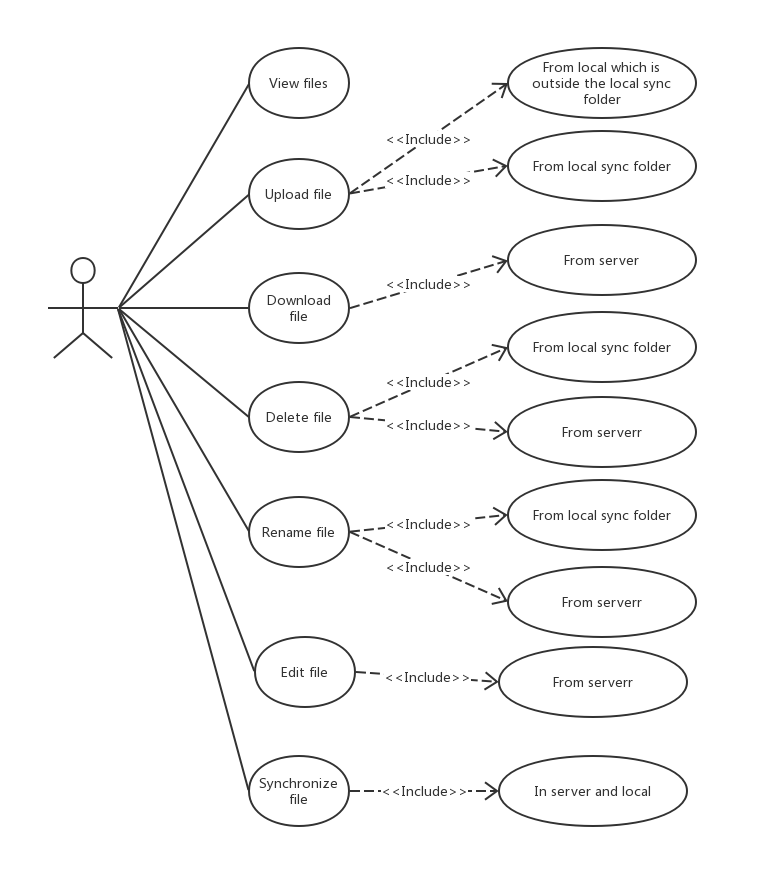
\includegraphics[scale=0.5]{User_use_case}

\caption{Functionalities provided by Deadline fighter application to Users}
\end{figure}

